\documentclass{beamer}


\usepackage[utf8]{inputenc}
\usepackage[frenchb]{babel}
\usepackage{verbatim}
\usepackage{graphicx}
	\graphicspath{{figures/}}
\usepackage{caption}
\usepackage{subcaption}
\usepackage{color}
\usepackage{amsmath}
\usepackage{amsfonts}
\usepackage{mathtools}
\usepackage{bm}

\usetheme{boxes}
\usefonttheme[onlymath]{serif}
\usecolortheme{beaver}
\beamertemplatenavigationsymbolsempty
\setbeamertemplate{title page}[default][colsep=-4bp,rounded=true]
\setbeamertemplate{sections/subsections in toc}[circle]
\setbeamertemplate{footline}[frame number]
\setbeamertemplate{itemize items}[circle]
\setbeamertemplate{itemize subitem}[square]
\setbeamertemplate{blocks}[rounded][shadow=false]
\setbeamercolor{block title}{bg=blue!40,fg=black}
\setbeamercolor{block body}{bg=blue!10,fg=black}

\newtheorem{important}{Important}
\newenvironment<>{important}[1][]{%
	\setbeamercolor{block title}{fg=white,bg=red!40!black}%
	\setbeamercolor{block body}{fg=black,bg=red!10}
	\setbeamertemplate{itemize item}{\color{red!40!black}$\blacktriangleright$}
	\begin{block}{#2}\textbf{#1}}{\end{block}}

\newcommand{\VecQSource}{{\bm{q}}}
\newcommand{\VecPosSource}{{\bm{x_s}}}
\newcommand{\VecTheta}{{\bm{\theta}}}
\newcommand{\VecObs}{{\bm{\eta}}}



\definecolor{lightgreen}{rgb}{0.0,0.8,0.0}
\definecolor{lightblue}{rgb}{0.3,0.8,1.0}
\definecolor{lightred}{rgb}{0.874,0.180,0.105}
\definecolor{gray}{rgb}{0.4,0.4,0.4}
\definecolor{lightgray}{rgb}{0.8,0.8,0.8}
\definecolor{shadecolor}{rgb}{0.9,0.9,0.9}




\title{Inférence bayésienne adaptative pour la reconstruction de source en dispersion atmosphérique}
\author{Harizo Rajaona}
\institute{Directeurs de thèse: Yves Delignon, François Septier}
% Put logos here!
\date{Lille \\ 21 novembre 2016}

\begin{document}
\AtBeginSection[]
{
	\begin{frame}
		\tableofcontents[currentsection]
		% Die Option [pausesections]
	\end{frame}
}
	
	
\begin{frame}
	\titlepage
\end{frame}
\begin{frame}
	\tableofcontents
\end{frame}

\section{Contexte et problématique}

% ===== Contexte (1) ================================================================
\begin{frame}
	\frametitle{Contexte}
	Les rejets \textbf{NRBC}\footnote{Nucléaires, Radiologiques, Biologiques, Chimiques} dans l'atmosphère peuvent être d'origine:
	\begin{itemize}
		\item accidentelle (fuite ou explosion sur un site industriel),
		\item malveillante (actes terroristes)
	\end{itemize}
	\begin{figure}
		\centering
		\begin{subfigure}[b]{0.33\textwidth}
			\centering
			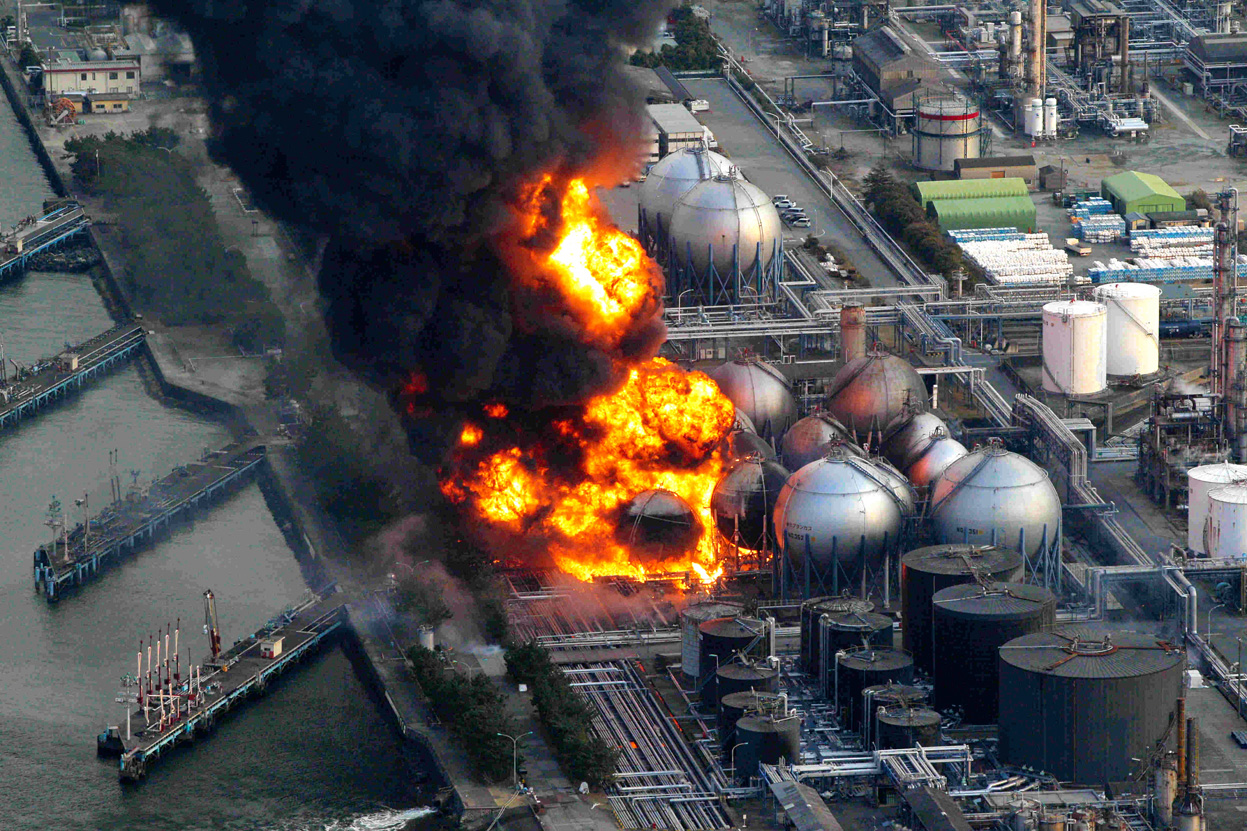
\includegraphics[width=\textwidth]{fukushima}
			\caption*{Fukushima (2011)}
		\end{subfigure}
		\hfill
		\begin{subfigure}[b]{0.3\textwidth}
			\centering
			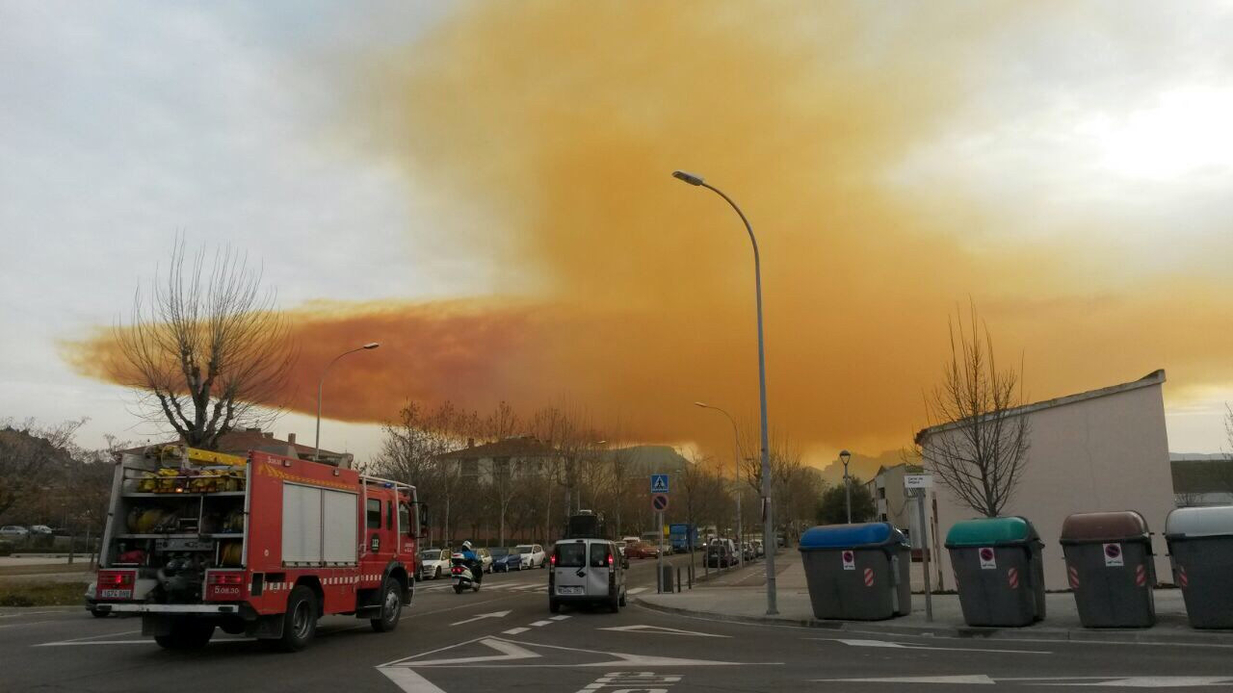
\includegraphics[width=\textwidth]{igualada}
			\caption*{Igualada (2015)}
		\end{subfigure}
		\hfill
		\begin{subfigure}[b]{0.3\textwidth}
			\centering
			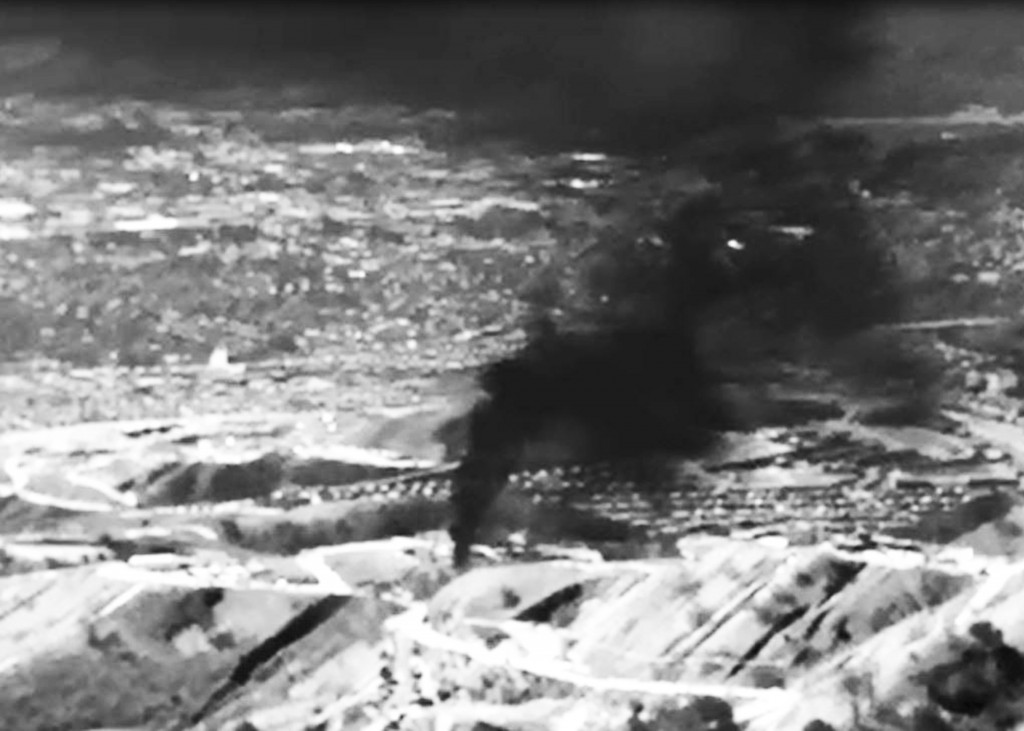
\includegraphics[width=\textwidth]{los_angeles}
			\caption*{Los Angeles (2015)}
		\end{subfigure}
	\end{figure}
	
	Durant de tels événements, les priorités sont alors:
	\begin{itemize}
		\item la mise en sécurité des populations,
		\item l'action des premiers secours pour atténuer/neutraliser le risque.
	\end{itemize}
\end{frame}

% ===== Contexte (2) ================================================================

\begin{frame}
	\frametitle{Contexte}
	Outils pour détecter et évaluer le risque:
	\begin{itemize}
		\item données d'observation (capteurs mesurant la concentration de polluant)
		\item outils de modélisation des phénomènes atmosphériques
	\end{itemize}
	\begin{figure}
		\centering
		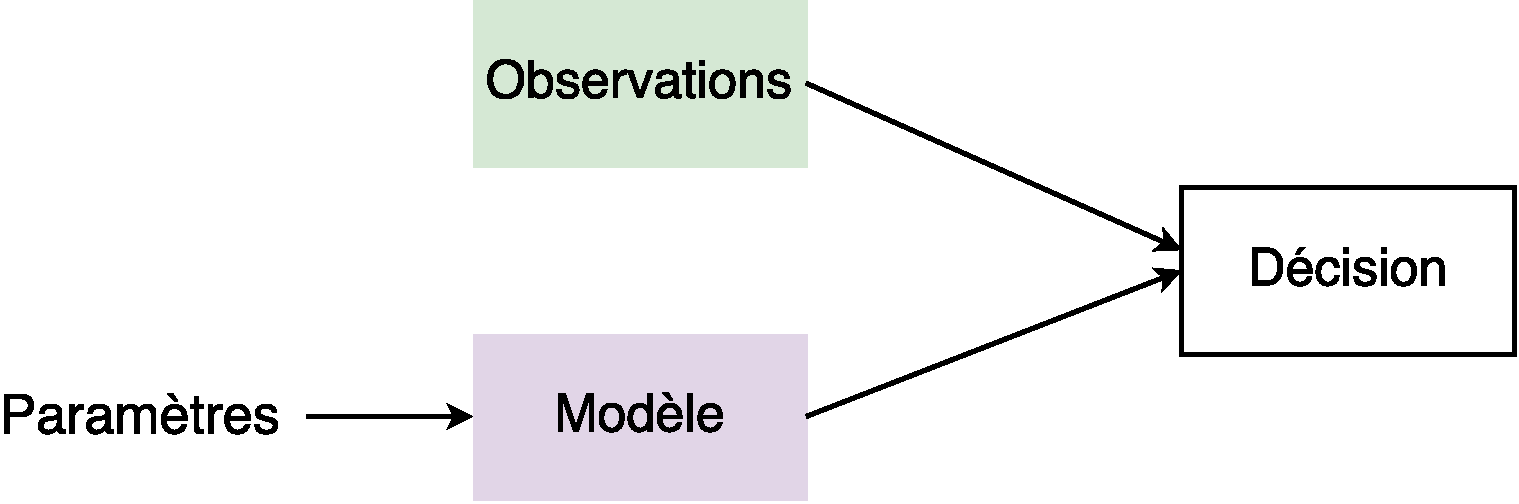
\includegraphics[width=0.9\textwidth]{diagram_context_2.pdf}
	\end{figure}
\end{frame}

% ===== Physique de l'atmosphère ================================================================

\begin{frame}
	\frametitle{Dispersion atmosphérique}
	\begin{block}{Modèle de dispersion}
		Outil de calcul numérique permettant de simuler la propagation dans l'atmosphère d'un rejet de polluant.
	\end{block}
	
	
	Typologie des modèles selon:
	\begin{itemize}
		\item  l'échelle (locale, régionale, synoptique),
		\item le degré de simplification des équations de la mécanique des fluides
	\end{itemize}
	
	Paramètres d'entrée:
	\begin{itemize}
		\item données météorologiques: vent (direction + vitesse), température, humidité, nébulosité, flux de rayonnement...
		\item terme source: position, quantités émises, durée, substance émise...
	\end{itemize}
\end{frame}

% =====  Terme source  ================================================================
\begin{frame}
	\frametitle{Terme source: définitions}
	Ici, on formule l'hypothèse d'une source:
	\begin{itemize}
		\item localisée (représentée par un point géographique $\VecPosSource \in \mathbb{R}^2$),
		\item unique (un seul point d'émission),
		\item non-instantanée (émission sur $T_s > 1$ intervalles de temps).\\
	\end{itemize}
	\vspace{0.3cm}
	Profil d'émission: vecteur $\VecQSource \in \mathbb{R}^{T_s} $:
		$$ \VecQSource = \left(q(t'_1), q(t'_2), \cdots, q(t'_{T_s})\right) $$
		
	\begin{figure}
		\centering
		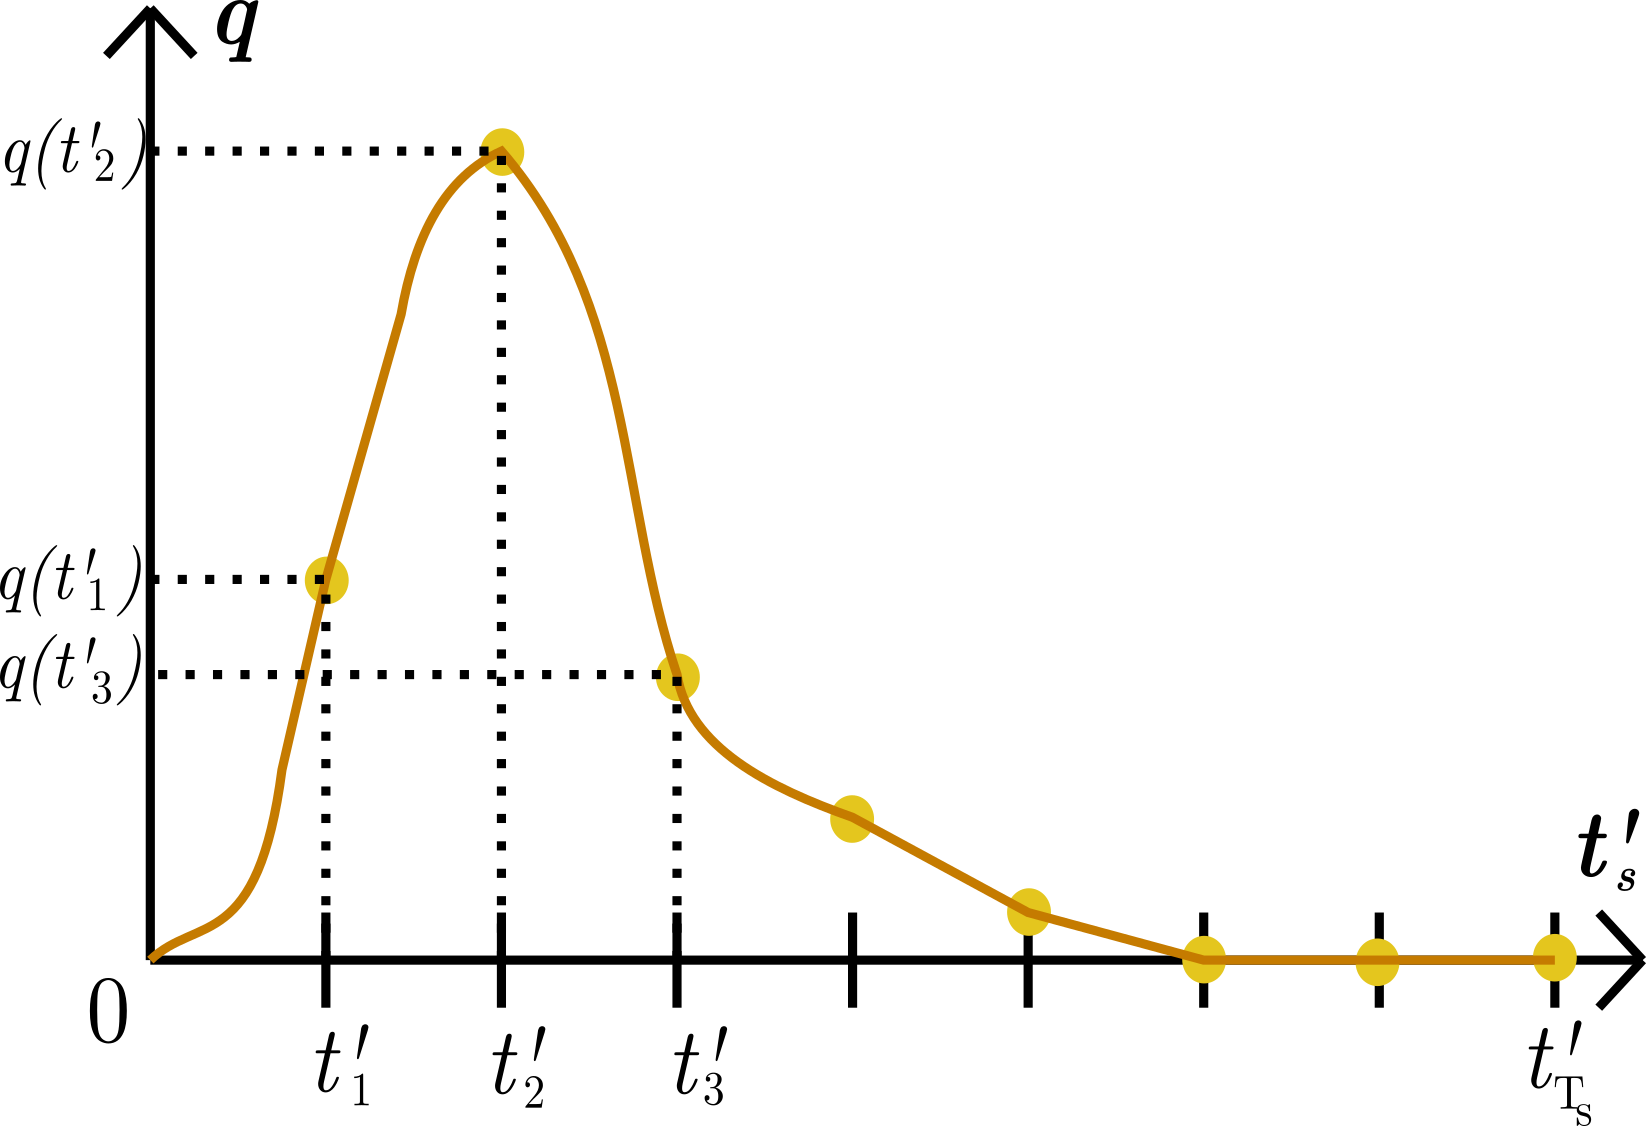
\includegraphics[width=0.6\textwidth]{courbe_profil_source}
	\end{figure}
	
\end{frame}

% =====  Terme source  ================================================================

\begin{frame}
	\frametitle{Terme source: estimation}
	Reconstruire les paramètres d'un terme source à partir des observations est un problème inverse.
	
	\begin{figure}
		\centering
		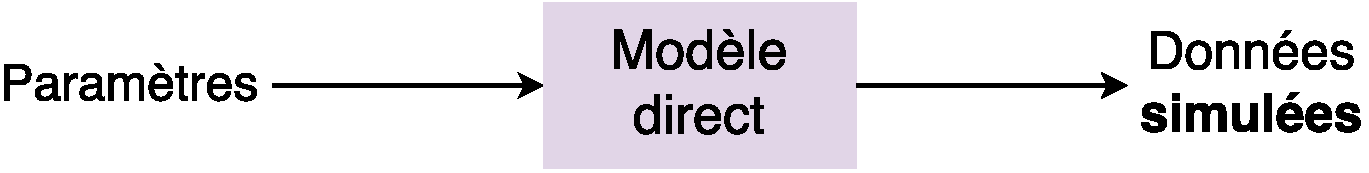
\includegraphics[width=0.75\textwidth]{modele_direct} \\
		\vspace{0.5cm}
		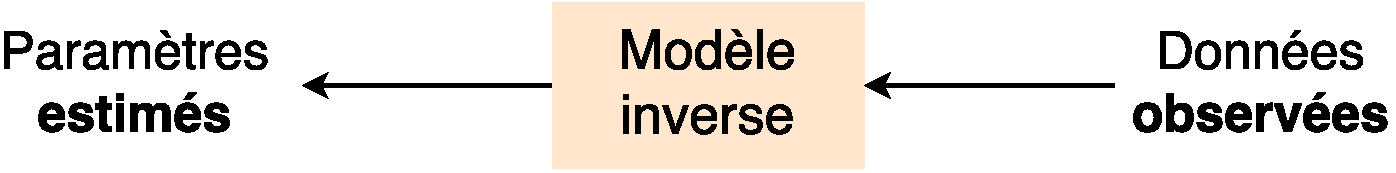
\includegraphics[width=0.75\textwidth]{modele_inverse}
	\end{figure}
	
	Plusieurs approches de résolution possibles:
	\begin{itemize}
		\item rétro-transport,
		\item résolution d'un système linéaire,
		\item algorithmes évolutionnaires,
		\item méthodes bayésiennes et simulation stochastique.
	\end{itemize}
\end{frame}


% =====  Problématique de recherche ================================================================

\begin{frame}
	\frametitle{Problématique de recherche}
	On se concentre sur les méthodes bayésiennes:
	\begin{itemize}
		\item formalisme rigoureux pour estimation et quantification de l'incertitude,
		\item exploitation d'un nombre limité de mesures (régularisation),
		\item {\color{red} temps de calcul potentiellement élevés,}
		\item {\color{red} estimation disjointe de la position et du profil d'émission.}
	\end{itemize}
	
    \begin{important}[Problématique:]
    	\begin{itemize}
    		\item Développer une méthode bayésienne pour estimer la localisation \textbf{et} le profil d'émission d'une source.
    		\item Coupler cette méthode avec un modèle de dispersion atmosphérique dans une chaîne de calcul opérationnelle.
    	\end{itemize}
    \end{important}
\end{frame}
% ++++++++++++++++++++++++++++++++++++++++++++++++++++++++++++++++++++++++
% ++++++++++++++++++++++++++++++++++++++++++++++++++++++++++++++++++++++++
\section{Une méthodologie adaptative pour l'inférence bayésienne}
% =====  Le choix bayésien ================================================================

\begin{frame}
	\frametitle{Le choix bayésien}
	\begin{block}{	Inférence bayésienne}
	Estimation probabiliste des paramètres $\VecTheta$ d'un système ayant généré un ensemble d'observations $\VecObs$.
	\end{block}
	\begin{itemize}
		\item $\VecTheta$: paramètres du terme source
		\item $\VecObs$: mesures de concentration observées
	\end{itemize}
	Règle de Bayes:
	$$ \pi(\VecTheta) = p(\VecTheta | \VecObs) = \dfrac{p(\VecTheta)p(\VecObs|\VecTheta)}{p(\VecObs)} \propto p(\VecTheta)p(\VecObs|\VecTheta) $$
	\begin{itemize}
		\item loi a posteriori $\pi(\VecTheta)$: information sur $\VecTheta$ après acquisition de $\VecObs$,
		\item loi a priori $p(\VecTheta)$: information préalable sur $\VecTheta$,
		\item fonction de vraisemblance $p(\VecObs | \VecTheta)$: probabilité d'observer $\VecObs$ pour $\VecTheta$ fixé.
	\end{itemize}
\end{frame}
% =====  Méthodes MC  ================================================================

\begin{frame}
	\frametitle{Le choix bayésien}
	\begin{itemize}
	\item \textbf{Problème}: $p(\VecObs | \VecTheta)$  trop coûteuse (ou impossible) à calculer \\$\Rightarrow$ {\color{red} pas d'expression analytique pour $p(\VecTheta | \VecObs)$ ! } \\
	
	 $\Rightarrow$ recours à des méthodes d'approximation numérique
	
	\begin{block}{Méthodes de Monte-Carlo}
		Permettent d'approximer l'espérance de toute fonction d'une variable aléatoire  de loi $\pi$:
%		\begin{equation*}
%			\begin{split}
%				\mathbb{E}_{\pi}[\psi(\VecTheta)] &= \int \psi(\VecTheta)\pi(\VecTheta)d\VecTheta \\
%				& \simeq \dfrac{1}{N} \sum\limits_{i=1}^{N}\psi(\theta^{(i)}), ~ ~ ~ \theta^{(i)} \sim \pi
%			\end{split}
%		\end{equation*}
		$$ \mathbb{E}_{\pi}[\psi(\VecTheta)] = \int \psi(\VecTheta)\pi(\VecTheta)d\VecTheta \simeq \dfrac{1}{N} \sum\limits_{i=1}^{N}\psi(\theta^{(i)}), ~ ~ ~ \theta^{(i)} \sim \pi $$
	\end{block}
	
	\item Estimateur bayésien MMSE: s'obtient en posant $\psi(\VecTheta) = \VecTheta$.
	
	\end{itemize}
	
	

\end{frame}

\section{Application au cas expérimental FFT07}
\begin{frame}
	(vide)
\end{frame}
\section{Application avec modèle rétrograde aux cas simulés Beaune et Opéra}
\begin{frame}
	(vide)
\end{frame}
\section{Conclusions et perspectives}
\begin{frame}
	(vide)
\end{frame}
\end{document}
